\exercisesheader{}

% 10 - ages_pennies_1

\eoce{\qt{Ages of pennies, Part I \label{ages_pennies_1}} The histogram below shows the distribution of ages of pennies at a bank. 

\noindent\begin{minipage}[c]{0.54\textwidth}
\begin{parts}
\item Describe the distribution.
\item Sampling distributions for means from simple random samples of 5, 30, and 100 pennies is shown in the histograms below. Describe the shapes of these distributions and comment on whether they look like what you would expect to see based on the Central Limit Theorem.
\end{parts}
\end{minipage}
\begin{minipage}[c]{0.44\textwidth}
\begin{center}
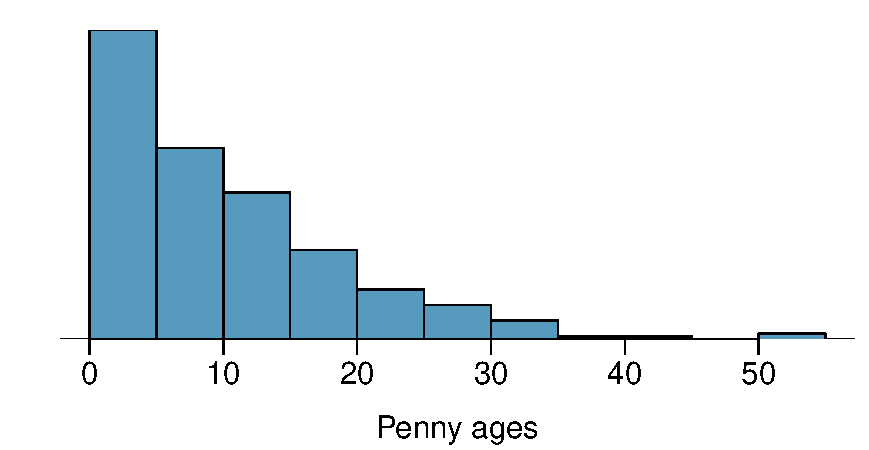
\includegraphics[width=\textwidth]{ch_distributions/figures/eoce/ages_pennies_1/penniesAges_pop} 
\end{center}
\end{minipage}\vspace{-1mm}
\begin{center}
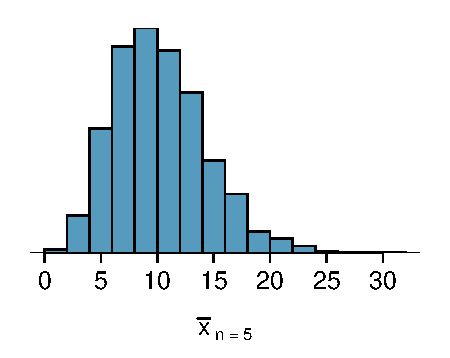
\includegraphics[width=0.325\textwidth]{ch_distributions/figures/eoce/ages_pennies_1/penniesAges_n5} 
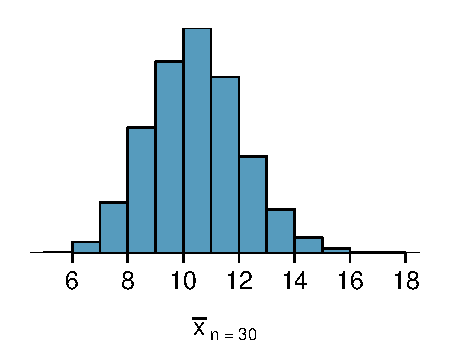
\includegraphics[width= 0.325\textwidth]{ch_distributions/figures/eoce/ages_pennies_1/penniesAges_n30} 
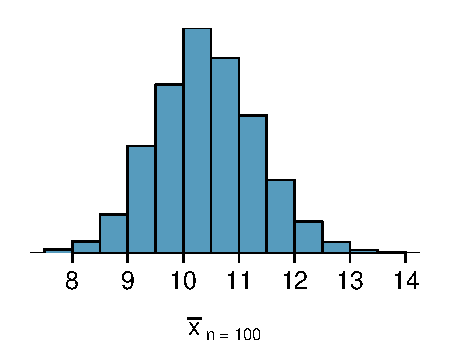
\includegraphics[width= 0.325\textwidth]{ch_distributions/figures/eoce/ages_pennies_1/penniesAges_n100} 
\end{center}
}{}

% 11 - ages_pennies_2

\eoce{\qt{Ages of pennies, Part II\label{ages_pennies_2}} The mean age of the pennies from Exercise~\ref{ages_pennies_1} is 10.44 years with a standard deviation of 9.2 years. Using the Central Limit Theorem, calculate the means and standard deviations of the distribution of the mean from random samples of size 5, 30, and 100. Comment on whether the sampling distributions shown in Exercise~\ref{ages_pennies_1} agree with the values you compute.
}{}

% 12 - housing_prices

\eoce{\qt{Housing prices\label{housing_prices}} \videosolution{ahss_eoce_sol-housing_prices} A housing survey was conducted to 
determine the price of a typical home in Topanga, CA. The mean price of a house 
was roughly \$1.3 million with a standard deviation of \$300,000. There were no 
houses listed below \$600,000 but a few houses above \$3 million.
\begin{parts}
\item Is the distribution of housing prices in Topanga symmetric, right skewed, 
or left skewed? \textit{Hint:} Sketch the distribution.
\item Would you expect most houses in Topanga to cost more or less than \$1.3 
million?
\item Can we estimate the probability that a randomly chosen house in Topanga 
costs more than \$1.4 million using the normal distribution?
\item What is the probability that the mean of 60 randomly chosen houses in 
Topanga is more than \$1.4 million?
\item How would doubling the sample size affect the standard deviation of the 
mean?
\end{parts}
}{}

% 13 - stats_final_scores

\eoce{\qt{Stats final scores\label{stats_final_scores}} Each year about 1500 students 
take the introductory statistics course at a large university. This year scores 
on the final exam are distributed with a median of 74 points, a mean of 70 
points, and a standard deviation of 10 points. There are no students who scored 
above 100 (the maximum score attainable on the final) but a few students scored 
below 20 points.
\begin{parts}
\item Is the distribution of scores on this final exam symmetric, right skewed, 
or left skewed?
\item Would you expect most students to have scored above or below 70 points?
\item Can we calculate the probability that a randomly chosen student scored 
above 75 using the normal distribution?
\item What is the probability that the average score for a random sample of 40 
students is above 75?
\item How would cutting the sample size in half affect the standard deviation of 
the mean?
\end{parts}
}{}

% 14 - identify_dist_symm_pop

\eoce{\qt{Identify distributions, Part I\label{identify_dist_symm_pop}} Four plots 
are presented below. The plot at the top is a distribution for a population. The 
mean is 10 and the standard deviation is 3. Also shown below is a distribution 
of (1) a single random sample of 100 values from this population, (2) a 
distribution of 100 sample means from random samples with size 5, and (3) a 
distribution of 100 sample means from random samples with size 25. Determine 
which plot (A, B, or C) is which and explain your reasoning.
\begin{center}
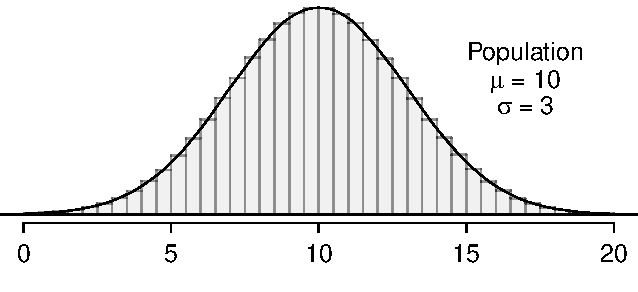
\includegraphics[width=0.55\textwidth]{ch_distributions/figures/eoce/identify_dist_symm_pop/identify_dist_symm_pop.pdf} \\
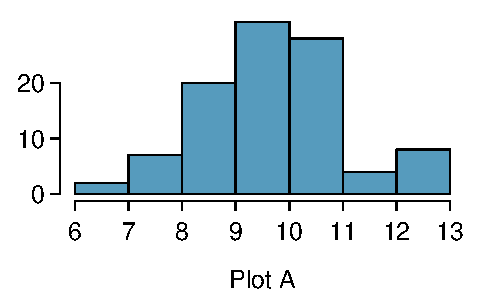
\includegraphics[width=0.325\textwidth]{ch_distributions/figures/eoce/identify_dist_symm_pop/identify_dist_symm_sampling_n5.pdf}
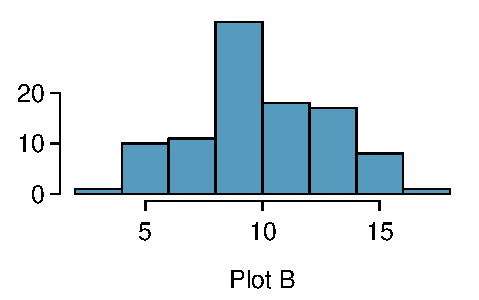
\includegraphics[width=0.325\textwidth]{ch_distributions/figures/eoce/identify_dist_symm_pop/identify_dist_symm_samp.pdf}
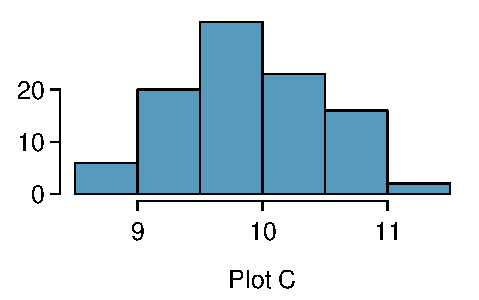
\includegraphics[width=0.325\textwidth]{ch_distributions/figures/eoce/identify_dist_symm_pop/identify_dist_symm_sampling_n25.pdf}
\end{center}
}{}

% 15 - identify_dist_ls_pop

\eoce{\qt{Identify distributions, Part II\label{identify_dist_ls_pop}} Four plots are presented below. The plot at 
the top is a distribution for a population. The mean is 60 and the standard 
deviation is 18. Also shown below is a distribution of (1) a single random 
sample of 500 values from this population, (2) a distribution of 500 sample 
means from random samples of each size 18, and (3) a distribution of 500 sample 
means from random samples of each size 81. Determine which plot (A, B, or C) is 
which and explain your reasoning.
\begin{center}
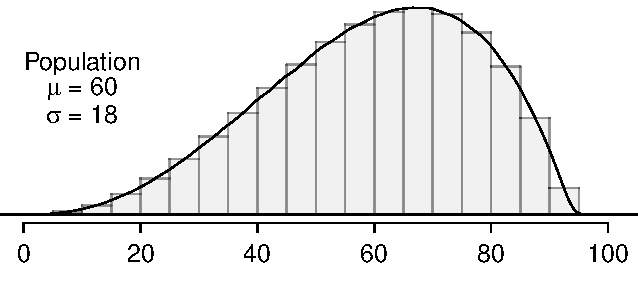
\includegraphics[width=0.55\textwidth]{ch_distributions/figures/eoce/identify_dist_ls_pop/identify_dist_ls_pop.pdf}
\end{center}
\begin{center}
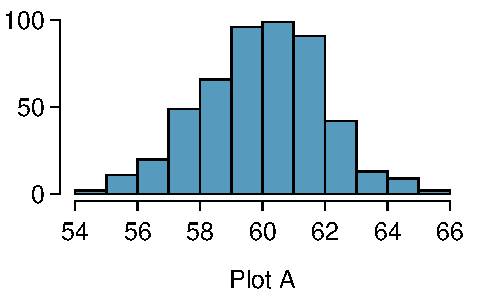
\includegraphics[width=0.325\textwidth]{ch_distributions/figures/eoce/identify_dist_ls_pop/identify_dist_ls_sampling_n81.pdf}
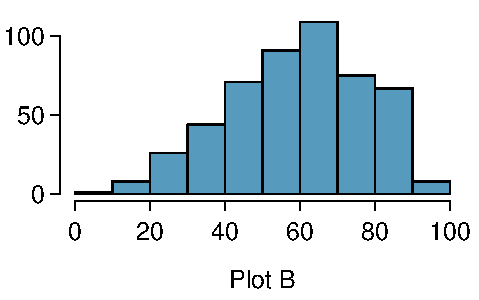
\includegraphics[width=0.325\textwidth]{ch_distributions/figures/eoce/identify_dist_ls_pop/identify_dist_ls_samp.pdf}
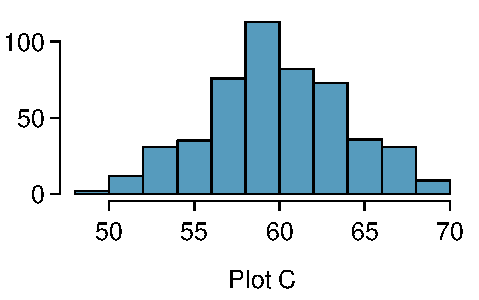
\includegraphics[width=0.325\textwidth]{ch_distributions/figures/eoce/identify_dist_ls_pop/identify_dist_ls_sampling_n18.pdf}
\end{center}
}{}

% 16 - penny_weights

\eoce{\qt{Weights of pennies\label{penny_weights}} The distribution of weights of 
United States pennies is approximately normal with a mean of 2.5 grams and a 
standard deviation of 0.03 grams.
\begin{parts}
\item What is the probability that a randomly chosen penny weighs less than 2.4 
grams?
\item Describe the sampling distribution of the mean weight of 10 randomly 
chosen pennies.
\item What is the probability that the mean weight of 10 pennies is less than 
2.4 grams?
\item Sketch the two distributions (population and sampling) on the same scale.
\item Could you estimate the probabilities from (a) and (c) if the weights of pennies had a skewed distribution?
\end{parts}
}{}

% 17 - cflbs

\eoce{\qt{CFLBs\label{cflbs}} A manufacturer of compact fluorescent light bulbs advertises 
that the distribution of the lifespans of these light bulbs is nearly normal with 
a mean of 9,000 hours and a standard deviation of 1,000 hours.
\begin{parts}
\item What is the probability that a randomly chosen light bulb lasts more than 
10,500 hours?
\item Describe the distribution of the mean lifespan of 15 light bulbs. 
\item What is the probability that the mean lifespan of 15 randomly chosen light 
bulbs is more than 10,500 hours?
\item Sketch the two distributions (population and sampling) on the same scale.
\item Could you estimate the probabilities from parts~(a) and~(c) if the 
lifespans of light bulbs had a skewed distribution?
\end{parts}
}{}

% 18 - songs_on_ipod

\eoce{\qt{Songs on an iPod\label{songs_on_ipod}} Suppose an iPod has 3,000 songs. The 
histogram below shows the distribution of the lengths of these songs. We also 
know that, for this iPod, the mean length is 3.45 minutes and the standard 
deviation is 1.63 minutes.
\begin{center}
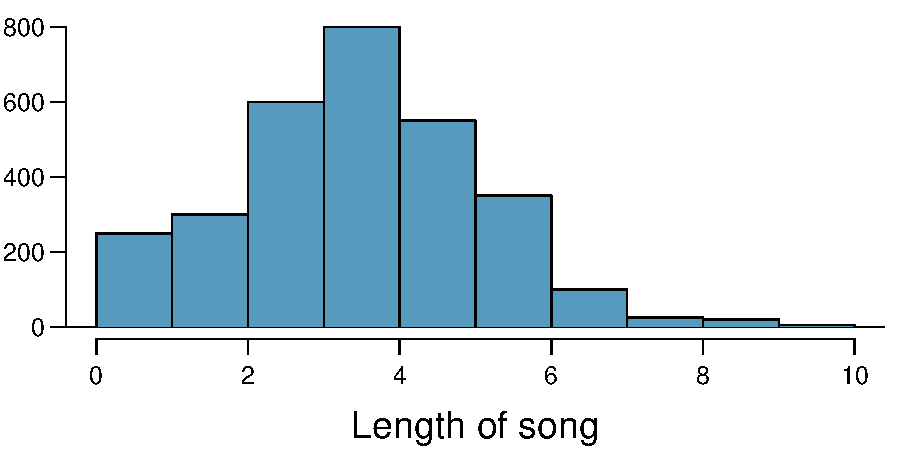
\includegraphics[width=0.5\textwidth]{ch_distributions/figures/eoce/songs_on_ipod/songs_on_ipod_pop_hist.pdf}
\end{center}
\begin{parts}
\item Calculate the probability that a randomly selected song lasts more than 5 
minutes.
\item You are about to go for an hour run and you make a random playlist of 15 songs. What is the probability that your playlist lasts for the entire duration 
of your run? \textit{Hint:} If you want the playlist to last 60 minutes, what should be the minimum average length of a song?
\item You are about to take a trip to visit your parents and the drive is 6 hours. You make a random playlist of 100 songs. What is the probability that your playlist lasts the entire drive?
\end{parts}
}{}

% 19 - spray_paint_2

\eoce{\qt{Spray paint, Part II\label{spray_paint_2}} Suppose the area that can be painted using a 
single can of spray paint is slightly variable and follows a nearly normal 
distribution with a mean of 25 square feet and a standard deviation of 3 square 
feet. 
\begin{parts}
\item What is the probability that the area covered by a can of spray paint is 
more than 27 square feet?
\item Suppose you want to spray paint an area of 540 square feet using 20 cans 
of spray paint. On average, how many square feet must each can be able to cover 
to spray paint all 540 square feet?
\item What is the probability that you can cover a 540 square feet area using 20 
cans of spray paint?
\item If the area covered by a can of spray paint had a slightly skewed 
distribution, could you still calculate the probabilities in parts~(a) and~(c) 
using the normal distribution?
\end{parts}
}{}

% 20 - wireless_routers

\eoce{\qt{Wireless routers\label{wireless_routers}} John is shopping for wireless routers and is overwhelmed by the number of available options. In order to get a feel for the average price, he takes a random sample of 75 routers and finds that the average price for this sample is \$75 and the standard deviation is \$25. 
\begin{parts}
\item Based on this information, how much variability should he expect to see in the mean prices of repeated samples, each containing 75 randomly selected wireless routers?
\item A consumer website claims that the average price of routers is \$80. Is a true average of \$80 consistent with John's sample?
\end{parts}
}{}

% 21 - betting_on_dinner_2

\eoce{\qt{Betting on dinner, Part II\label{betting_on_dinner_2}} Exercise~\ref{betting_on_dinner_1} introduces a promotion at a restaurant where prices of menu items are determined randomly following some underlying distribution. We are told that the price of basket of fries is drawn from a normal distribution with mean 6 and standard deviation of 2. You want to get 5 baskets of fries but you only have \$28 in your pocket. What is the probability that you would have enough money to pay for all five baskets of fries?
}{}
